\section{电压}\label{sec:8-3}

\xiaobiaoti{电压}
导体内有大量可以自由移动的电荷,在导体没有连入电路时,
导体内的这些自由电荷只做无规则的热运动,并不发生定向移动而形成电流。
例如,一盏电灯在没有和电源连通时不亮,表明这时电路里没有电流。
而当它和电源连通时就亮了,表明这时电路里有了电流。
那么,电源为什么能使导体中的自由电荷定向移动而形成电流呢?
我们对照水流的情形来理解这个问题。

在图 \ref{fig:8-8} 所示的连通器里,如果打开阀门 $K$,水路畅通,就会形成由 $A$ 经 $C$ 向 $B$ 的水流。
水所以能发生定向移动,是因为 $A$ 槽的水位高,$B$ 槽的水位低,从而在连接 $A$、$B$ 的水管中产生了水压。
水压是使水发生定向移动形成水流的原因。
\begin{figure}[htbp]
    \centering
    \begin{minipage}{7cm}
    \centering
    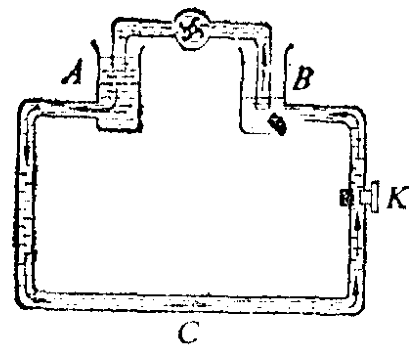
\includegraphics[width=6cm]{../pic/czwl2-ch8-8}
    \caption{水流的形成}\label{fig:8-8}
    \end{minipage}
    \qquad
    \begin{minipage}{7cm}
    \centering
    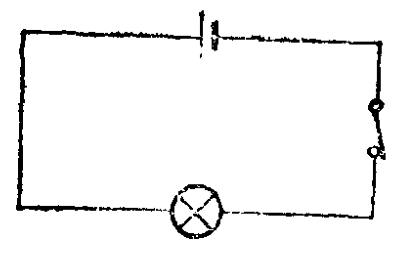
\includegraphics[width=6cm]{../pic/czwl2-ch8-9}
    \caption{}\label{fig:8-9}
    \end{minipage}
\end{figure}
与此相似,在图 \ref{fig:8-9} 里,电键闭合后,电路里就有电流。
电路里的自由电荷所以能发生定向移动形成电流,是因为电源的正极有多余的正电荷,
电源的负极有多余的负电荷,从而在连接电源两极的电路中产生了电压。
\CJKunderwave{电压是使自由电荷发生定向移动形成电流的原因}。

在图 \ref{fig:8-8} 中,如果用抽水机不断地把水从 $B$ 处抽到 $A$ 处,使 $A$ 处的水位总比 $B$ 处的高,
保持一定的水压,在连通器里就不断有水流通过。
电源的作用跟抽水机相似,它不断使正极聚集正电荷,负极聚集负电荷,
保持两极间的一定的电压,使连接导体中不断有电流通过。

水在流动的时候可以做功,例如水流可以推动水轮机做功。
水流做的功,除了跟流过的水量有关系外,还跟水压有关系。
流过的水量越多,水压越大,水流所做的功就越多。
电流在通过导体时也要做功,如电流通过白炽电灯做功,使灯泡发热发光,
电流通过电动机做功,使电动机运转。
电流做功跟水流做功也很相似,除了跟电量有关外,还跟电压有关。
通过的电量越多,电压越大,电流所做的功就越多。

既然电流做的功跟电压有关系,在电学里就利用电流所做的功来规定电压的单位。

电压的单位是\textbf{伏特}。
\CJKunderwave{在某段电路上每通过 1 库仑电量的时候,电流所做的功如果是 1 焦耳,这段电路两端的电压就是 1 伏特}。
伏特的符号是 V。

一节干电池的电压是 1.5 伏特,这就是说,在由一节干电池作电源的电路里,
每通过 1 库仑电量时, 电流做 1.5 焦耳的功。

比伏特大的单位有千伏(kV),比伏特小的单位有毫伏(mV)、微伏($\mu$V)。
\begin{align*}
    1 \text{千伏} &= 1000 \text{伏特,}\\
    1 \text{伏特} &= 1000 \text{毫伏,}\\
    1 \text{毫伏} &= 1000 \text{微伏。}\\
\end{align*}

\begin{table}[H]
    \centering
    \caption*{一些电压值 (伏特)}
    \begin{tabular}{w{l}{10em}w{r}{10em}}
        电子手表用的氧化银电池      & $1.5$ \\
        干电池组($n$ 节串联)      & $n \times 1.5$ \\
        铅蓄电池组($n$ 个串联)    & $n \times 2$ \\
        汽车发电机                 & $12$ \\
        对人体安全的电压            & 不高于 $36$ \\
        照明电路                    & $220$ \\
        一般交流电动机              & $220$,$380$ \\
        大型发电机                  & $(0.63\text{~}1.8) \times 10^4$ \\
        发生闪电的云层间的电压      & 可达 $10^8$ \\
    \end{tabular}
\end{table}



\xiaobiaoti{伏特表}
测量电压要使用电压表。刻度盘上以伏特为单位的电压表,标着一个字母 V,通常叫伏特表(图 \ref{fig:8-10})。

\begin{figure}[htbp]
    \centering
    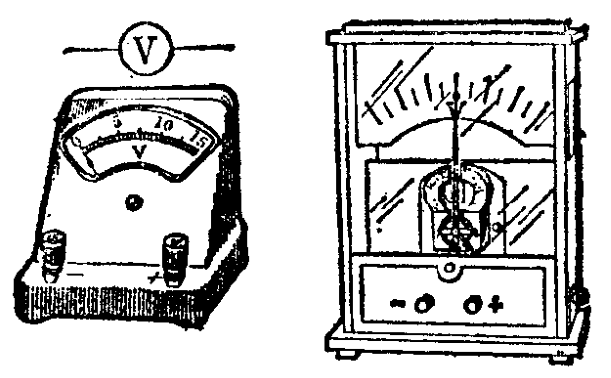
\includegraphics[width=0.7\textwidth]{../pic/czwl2-ch8-10}
    \caption{伏特表(左图上方是伏特表符号)}\label{fig:8-10}
\end{figure}

如果要测量某部分电路两端的电压,例如要测量图 \ref{fig:8-11} 中小灯泡 $L_2$ 两端的电压,
\CJKunderwave*{必须把伏特表跟这部分电路并联,并必须把伏特表 “$+$” 接线柱接在跟电源正极相连的那端}。

\begin{figure}[htbp]
    \centering
    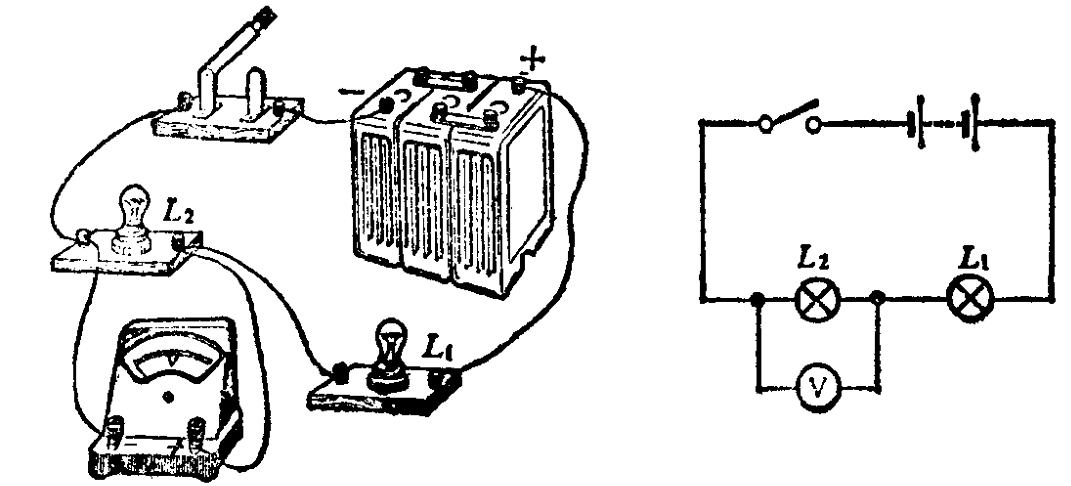
\includegraphics[width=0.7\textwidth]{../pic/czwl2-ch8-11}
    \caption{}\label{fig:8-11}
\end{figure}

每个伏特表都有一定的测量范围——量程,使用时必须注意所测的电压得超过伏特表的量程。

